\documentclass[]{article}

\usepackage{amsmath,amssymb,amsbsy}
\usepackage[letterpaper,total={6in,8in}]{geometry}
\usepackage[colorlinks]{hyperref}

\ifpdf
  \RequirePackage{graphicx}
  \RequirePackage{epstopdf}
  \DeclareGraphicsExtensions{.pdf,.jpeg,.png,.jpg}
\else
  \RequirePackage[dvipdfmx]{graphicx}
  \RequirePackage{bmpsize}
  \DeclareGraphicsExtensions{.eps,.pdf,.jpeg,.png,.jpg}
\fi
\graphicspath{{pics/},}
\RequirePackage{subfigure}
\providecommand{\subfigureautorefname}{\figureautorefname}

%opening
\title{Data Report for ``Multichannel Deconvolution of Skin Conductance Data: Concurrent Separation of Tonic and Phasic Component''}
\author{Yuchen Jin, Jin Lu}

\begin{document}

\maketitle

The dataset used for this project is called \texttt{PsPM-SCRV10}\cite{bach2014pspm}, where ``\texttt{PsPM}'' is the abbreviation of the organization ``Psycho-Physiological Modelling'', and ``\texttt{SCRV\_10}'' is the symbolic name of the dataset. This dataset is collected from an experiment. 26 volunteers (12 males and 14 females) are invited for participating the test. The researchers produce a series white noise bursts. In response, the participants are required to press food pedals every time they hear the burst. The data is recorded by Cambridge Electronic Design (CED) spike software.

According to the type of the data, the dataset could be divided into two parts. The first part is called ``cogent''. It contains the record about the participants' reactions including which pedal they press and how long the pedal is pressed. This part is not related to our work. The second part is called ``spikes''. It is a collection of skin conductance response (SCR) measurements including:

\begin{enumerate}
  \item Markers for when the loud sounds burst;
  \item Skin conductance on the thenar/hypothenar of the non-dominant hand;
  \item Skin conductance on the volar middle phalanx of the dominant 2nd/3rd finger;
  \item Skin conductance on the medial plantar surface of the non-dominant foot;
  \item Markers for heart beats;
  \item Respiration;
\end{enumerate}

In this report, we will inspect on the above 6 kinds of data in the raw set. We will also show some results produced by the codes from the work of \textit{Amin and Faghih}~\cite{amin2019robust}.

\section{Inspection on the raw dataset}

The dataset contains records for 731.7 seconds. First, we design a function \texttt{show\_raw\_dataset} for showing the raw dataset. The codes could be found in the Github project~\cite{jin2020}. In the following part, we will show all of the results respectively.

In the following part, we take the $6^{\mathrm{th}}$ data as an example. As shown in \autoref{fig:raw-marks}, channel 1 provides the exact time when the loud sound presents. The loud sound will happen about one minute after the measurement begins. The time interval between two sounds is about 30 seconds. Total number of sound events is 20 and the measurement duration is more than 700 seconds. 

\begin{figure}[htbp]
  \centering
  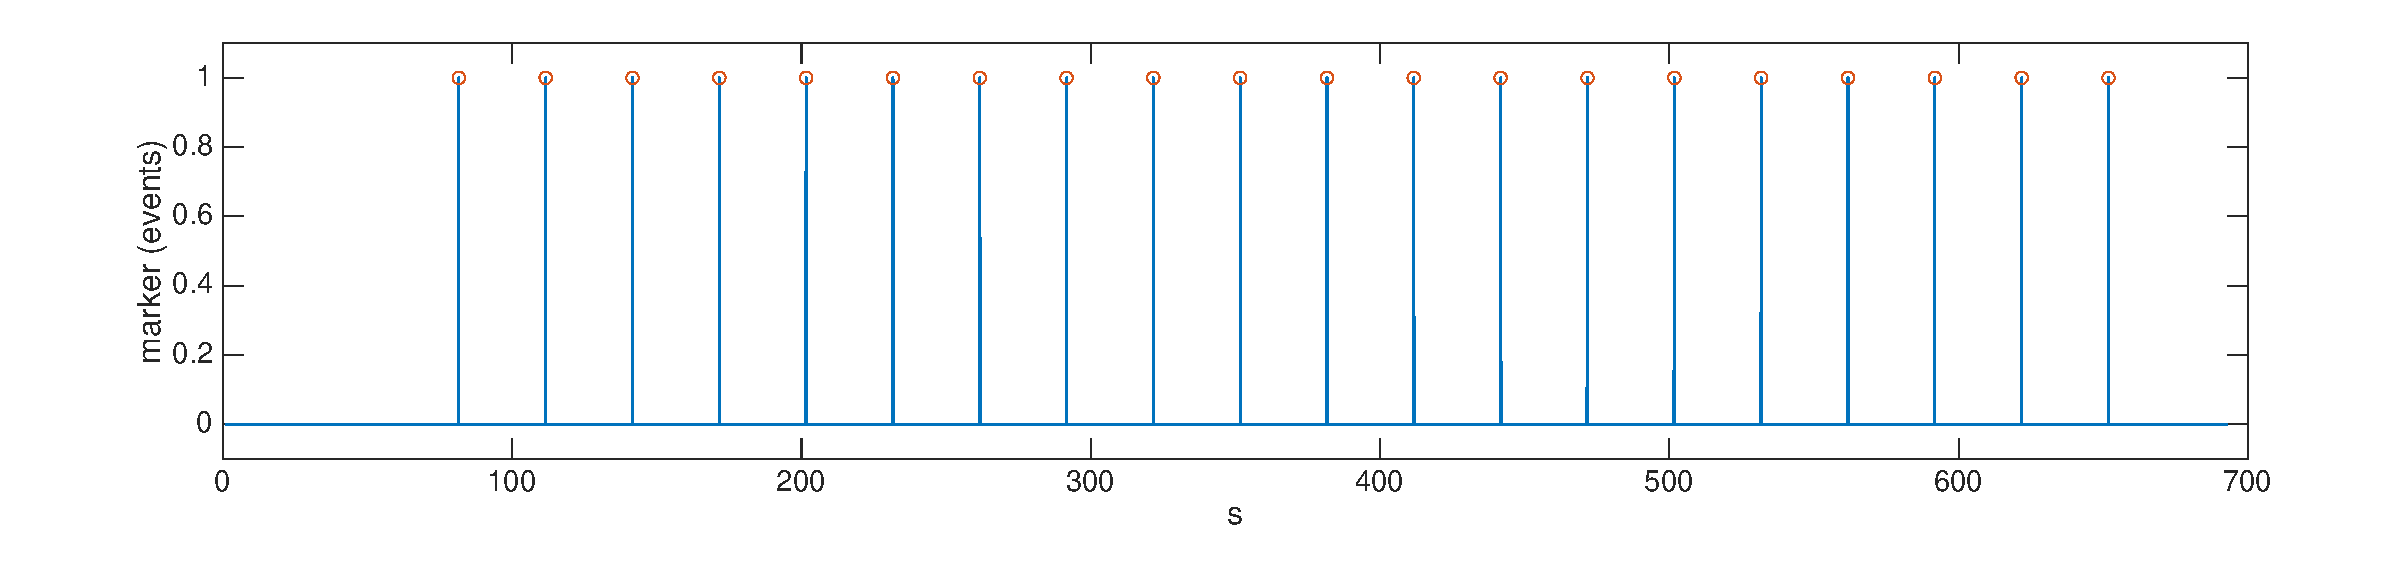
\includegraphics[width=0.9\textwidth]{data/raw-marks}
  \DeclareGraphicsExtensions.
  \caption{The marks for the loud sound presents.} \label{fig:raw-marks}
\end{figure}

Channel 2,3,4 are all Galvanic Skin Response (GSR) channels. \autoref{fig:raw-thenar}, \autoref{fig:raw-volar} and \autoref{fig:raw-medial} show the three different time series collected in different locations. Especially, since there is obvious outliers in \autoref{fig:raw-medial}, we plot another figure properly zoomed.

\begin{figure}[htbp]
  \centering
  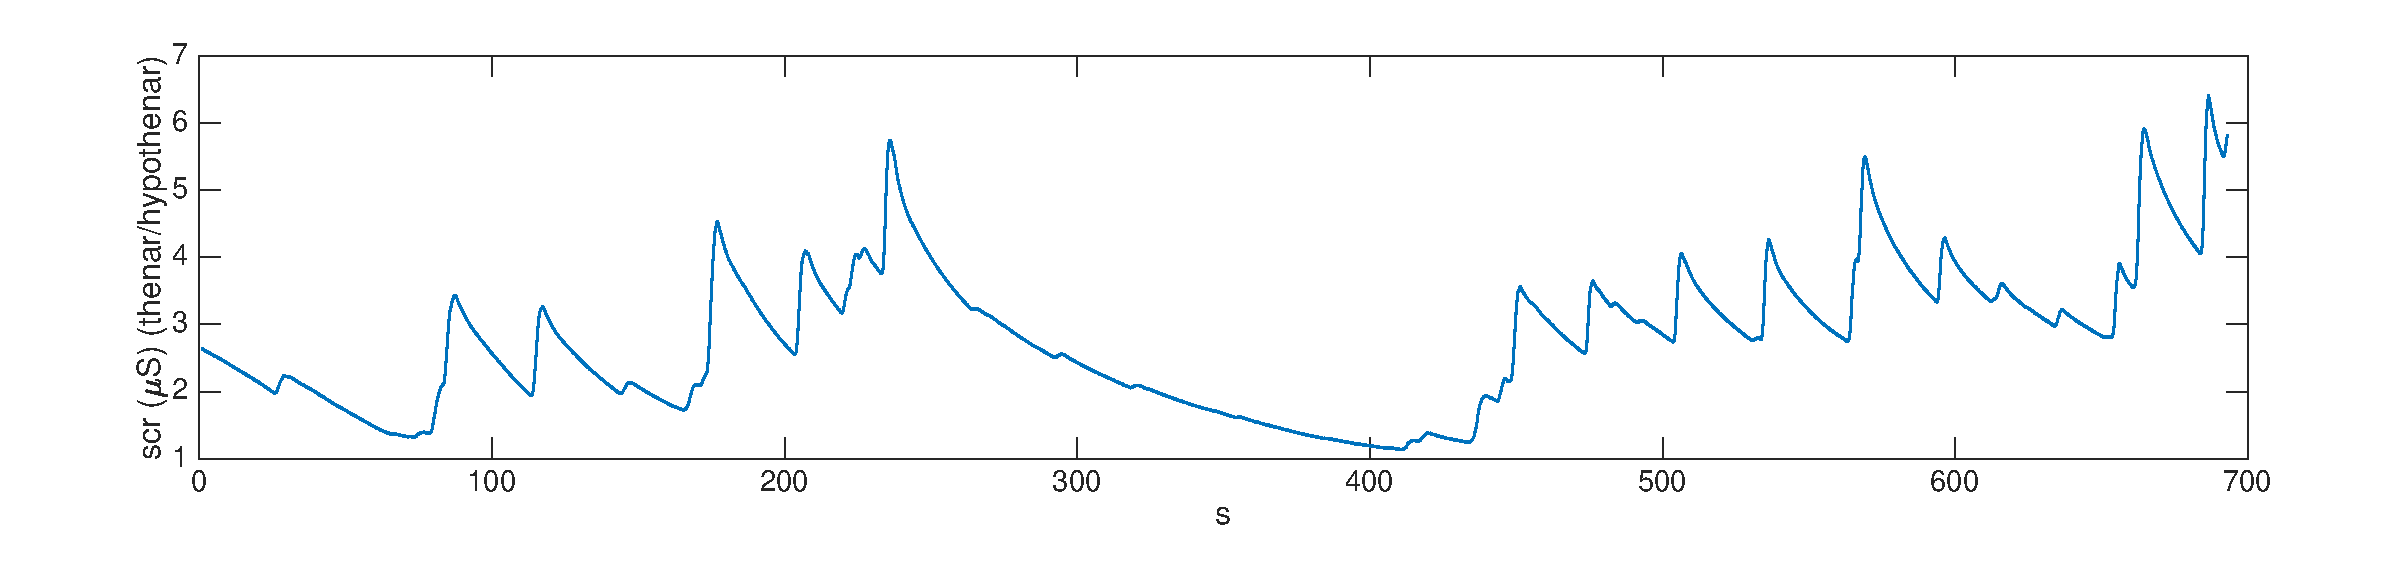
\includegraphics[width=0.9\textwidth]{data/raw-thenar}
  \DeclareGraphicsExtensions.
  \caption{GSR on the thenar/hypothenar of the non-dominant hand.} \label{fig:raw-thenar}
\end{figure}

\begin{figure}[htbp]
  \centering
  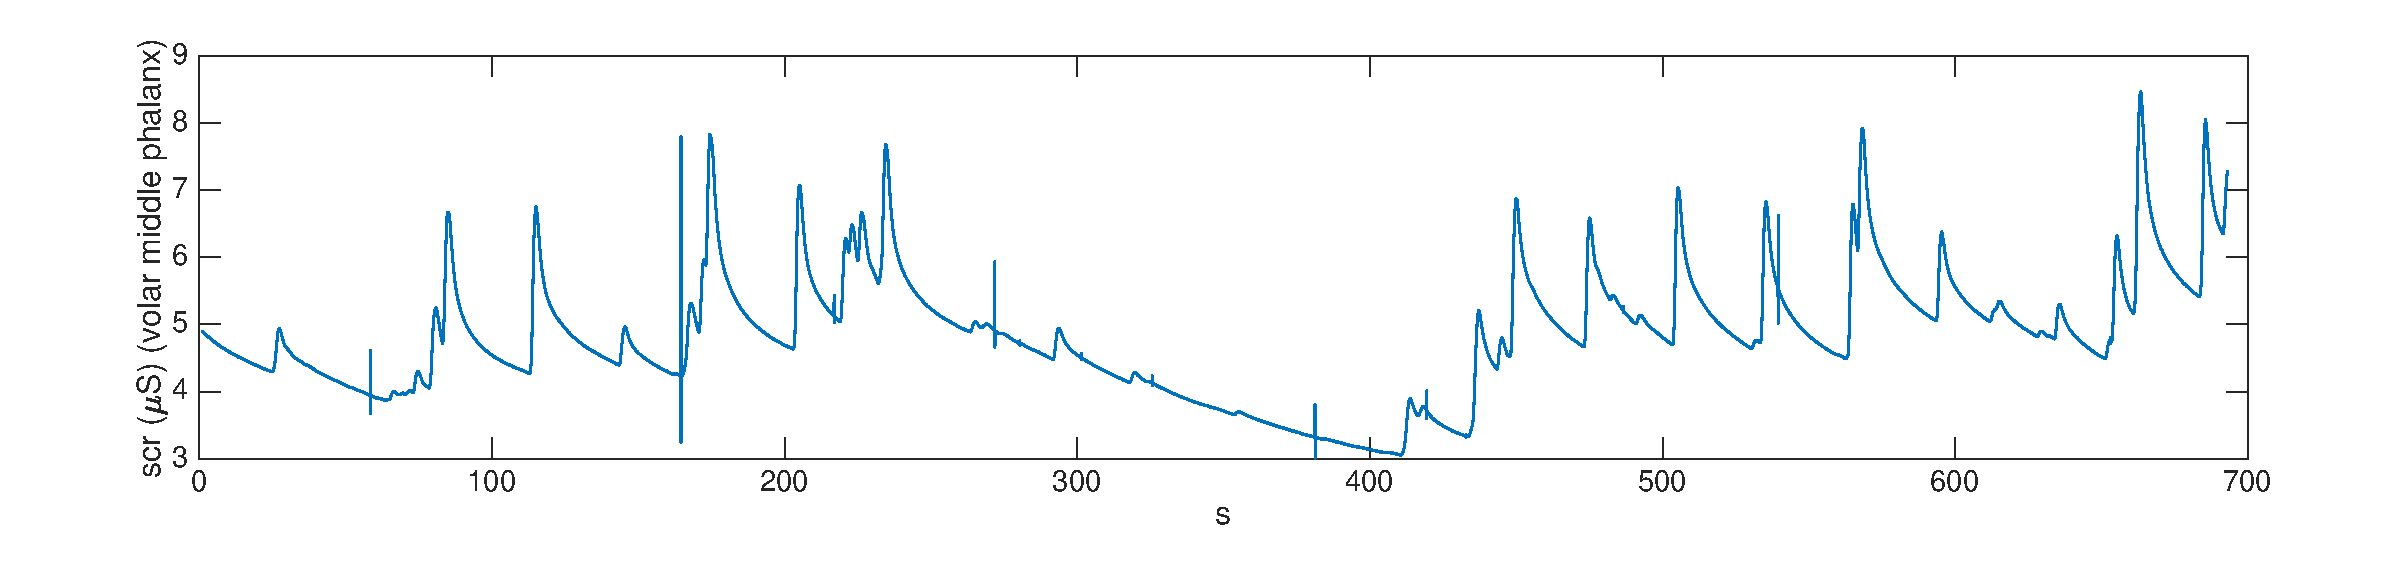
\includegraphics[width=0.9\textwidth]{data/raw-volar}
  \DeclareGraphicsExtensions.
  \caption{GSR on the volar middle phalanx of the dominant 2nd/3rd finger.} \label{fig:raw-volar}
\end{figure}

\begin{figure}[htbp]
  \centering
  \subfigure[Raw data.]{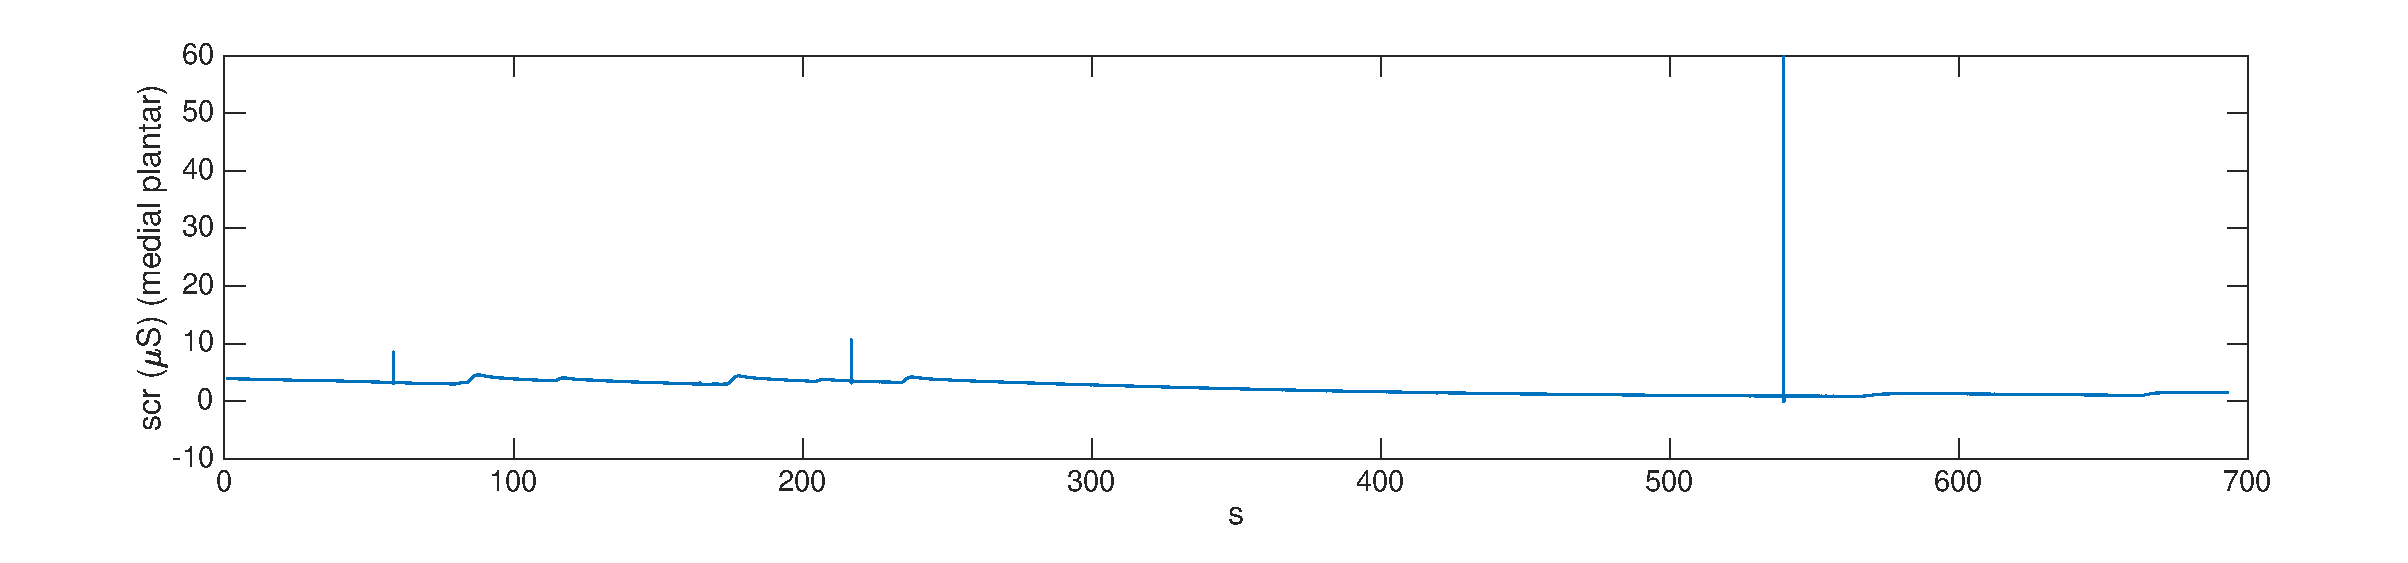
\includegraphics[width=0.9\textwidth]{data/raw-medial-2}}
  \subfigure[Zoomed data.]{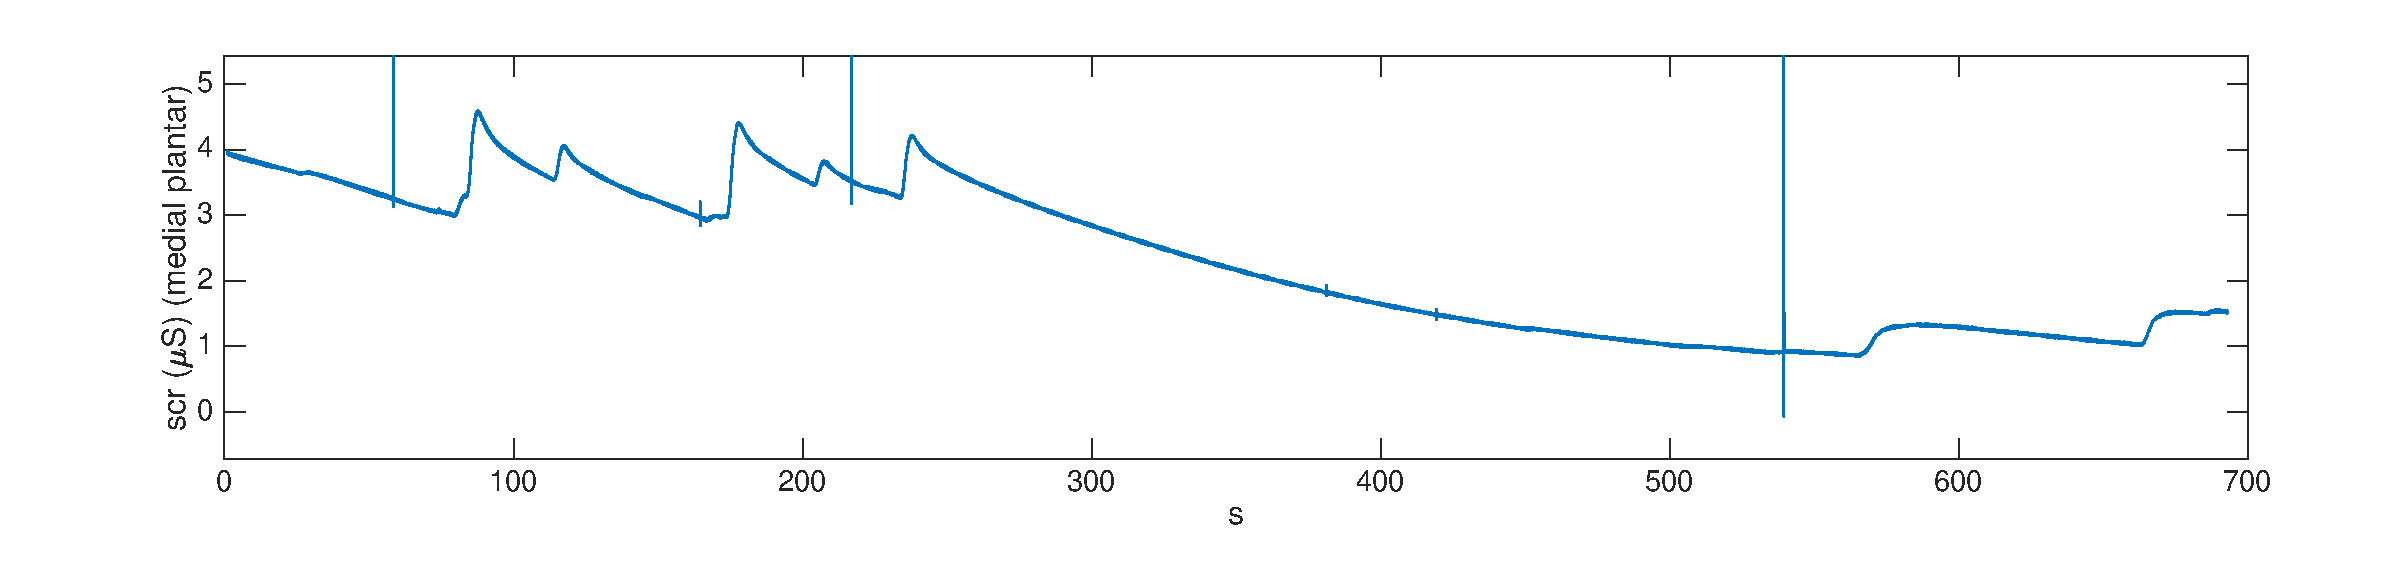
\includegraphics[width=0.9\textwidth]{data/raw-medial}}
  \DeclareGraphicsExtensions.
  \caption{GSR on the medial plantar surface of the non-dominant foot.} \label{fig:raw-medial}
\end{figure}

\autoref{fig:raw-thenar} shows the fifth channel containing heart beat signal. It provides the exact time when a heart beat happens. The heart beat is regular and dense with respect to the distribution in 700 seconds. To inspect on it more clearly, we show a zoomed figure in the range of $[100,200]\mathrm{s}$.

\begin{figure}[htbp]
  \centering
  \subfigure[From 0s to 700s.]{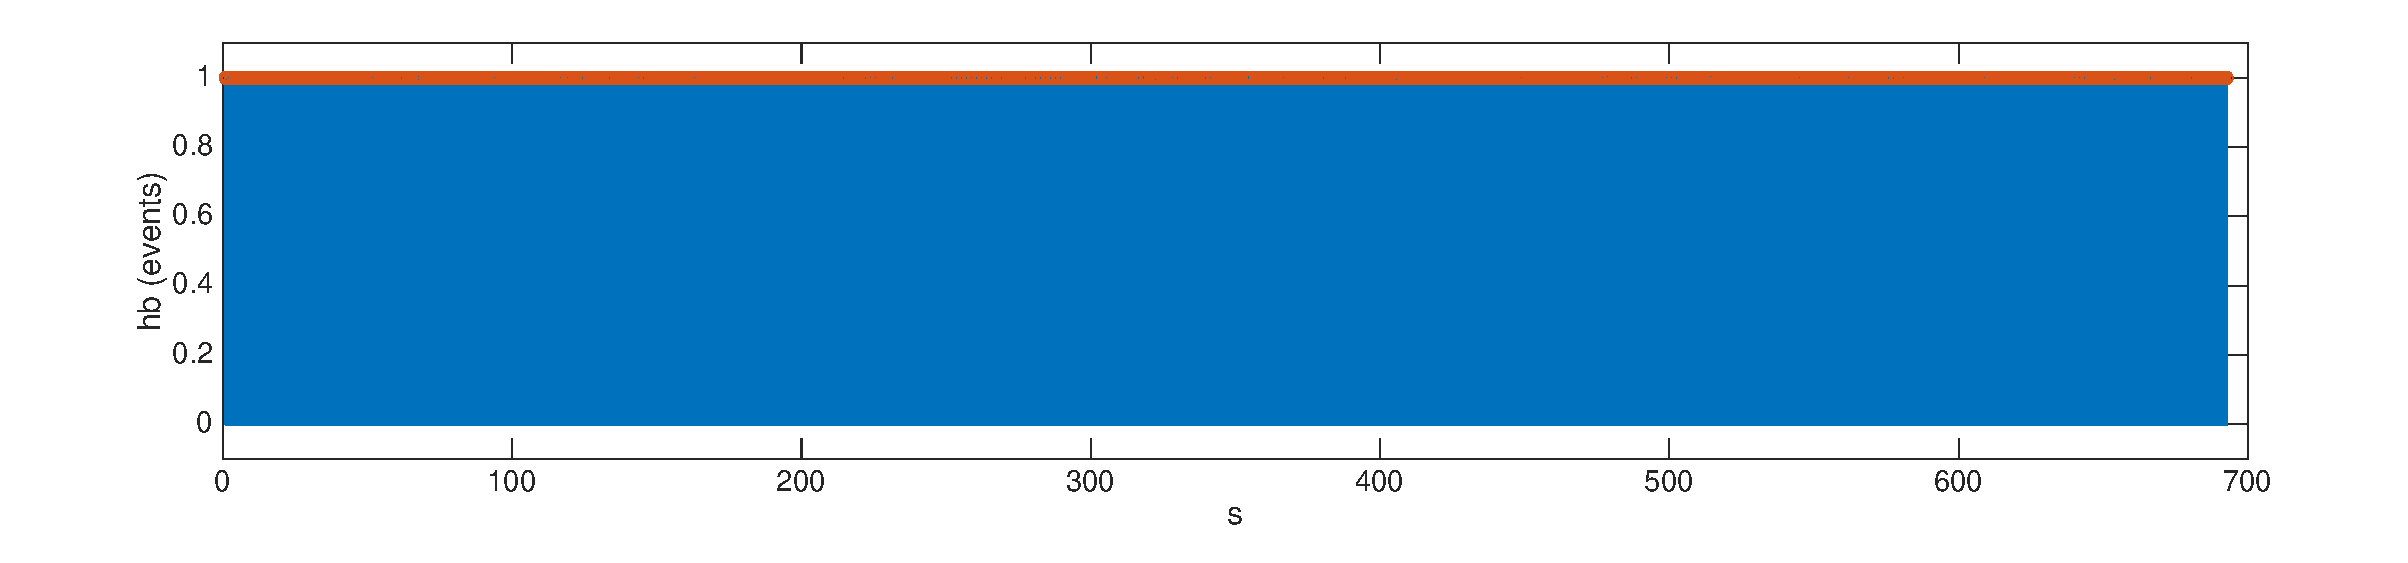
\includegraphics[width=0.9\textwidth]{data/raw-hb}}
  \subfigure[From 100s to 200s.]{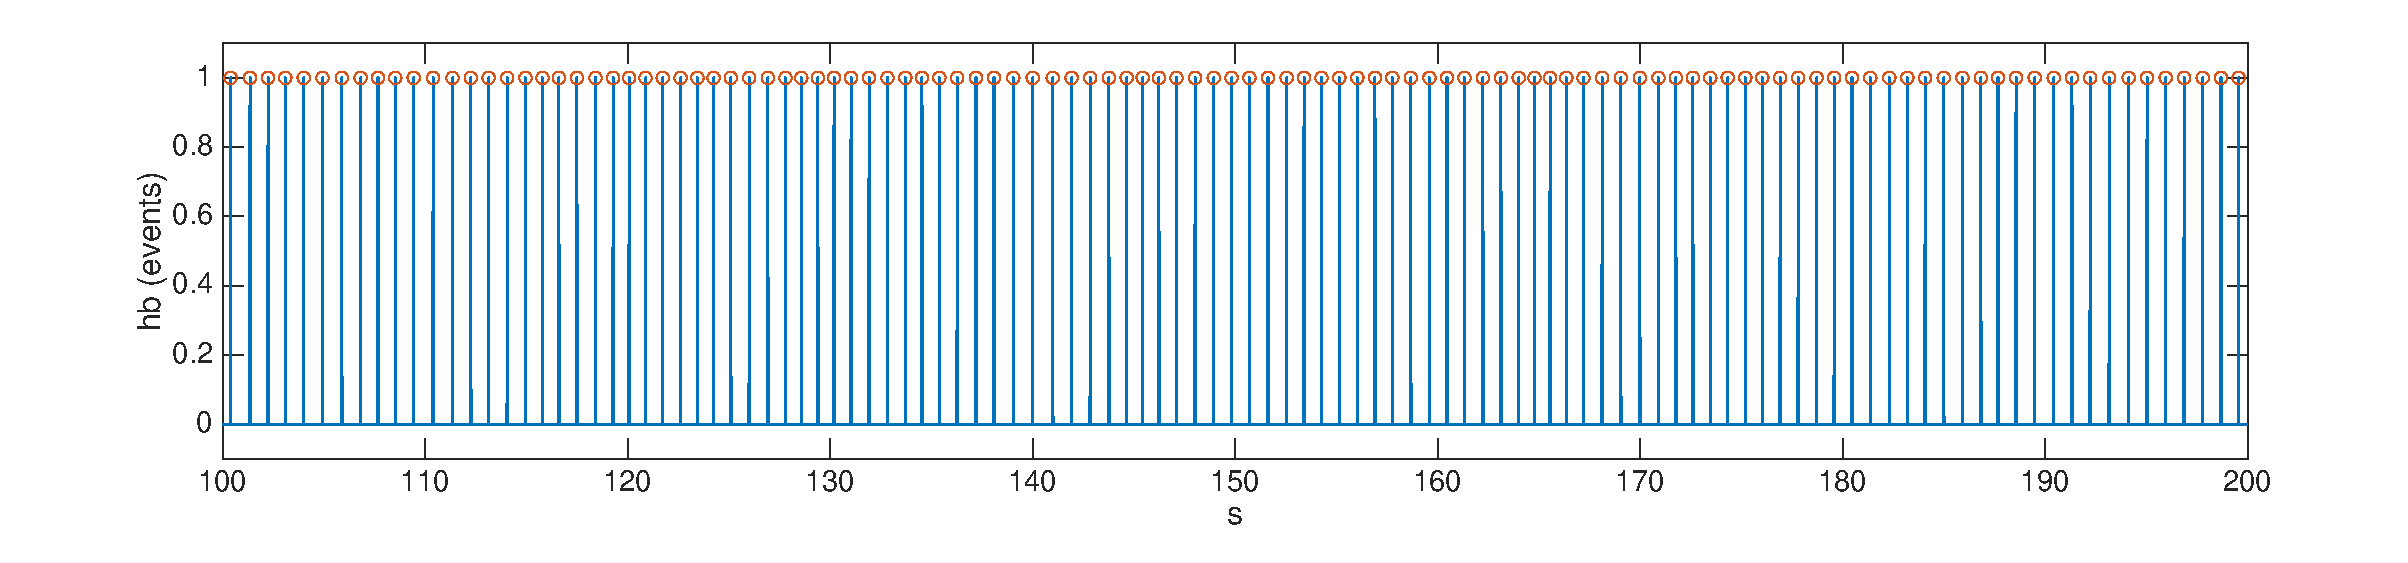
\includegraphics[width=0.9\textwidth]{data/raw-hb-2}}
  \DeclareGraphicsExtensions.
  \DeclareGraphicsExtensions.
  \caption{The marks for heart beats.} \label{fig:raw-hb}
\end{figure}

The last channel is the respiration signal. We show the signal in \autoref{fig:raw-resp}. According to the dataset description~\cite{bach2014pspm}, both the heart beat signal and the respiration signal may be incomplete.

\begin{figure}[htbp]
  \centering
  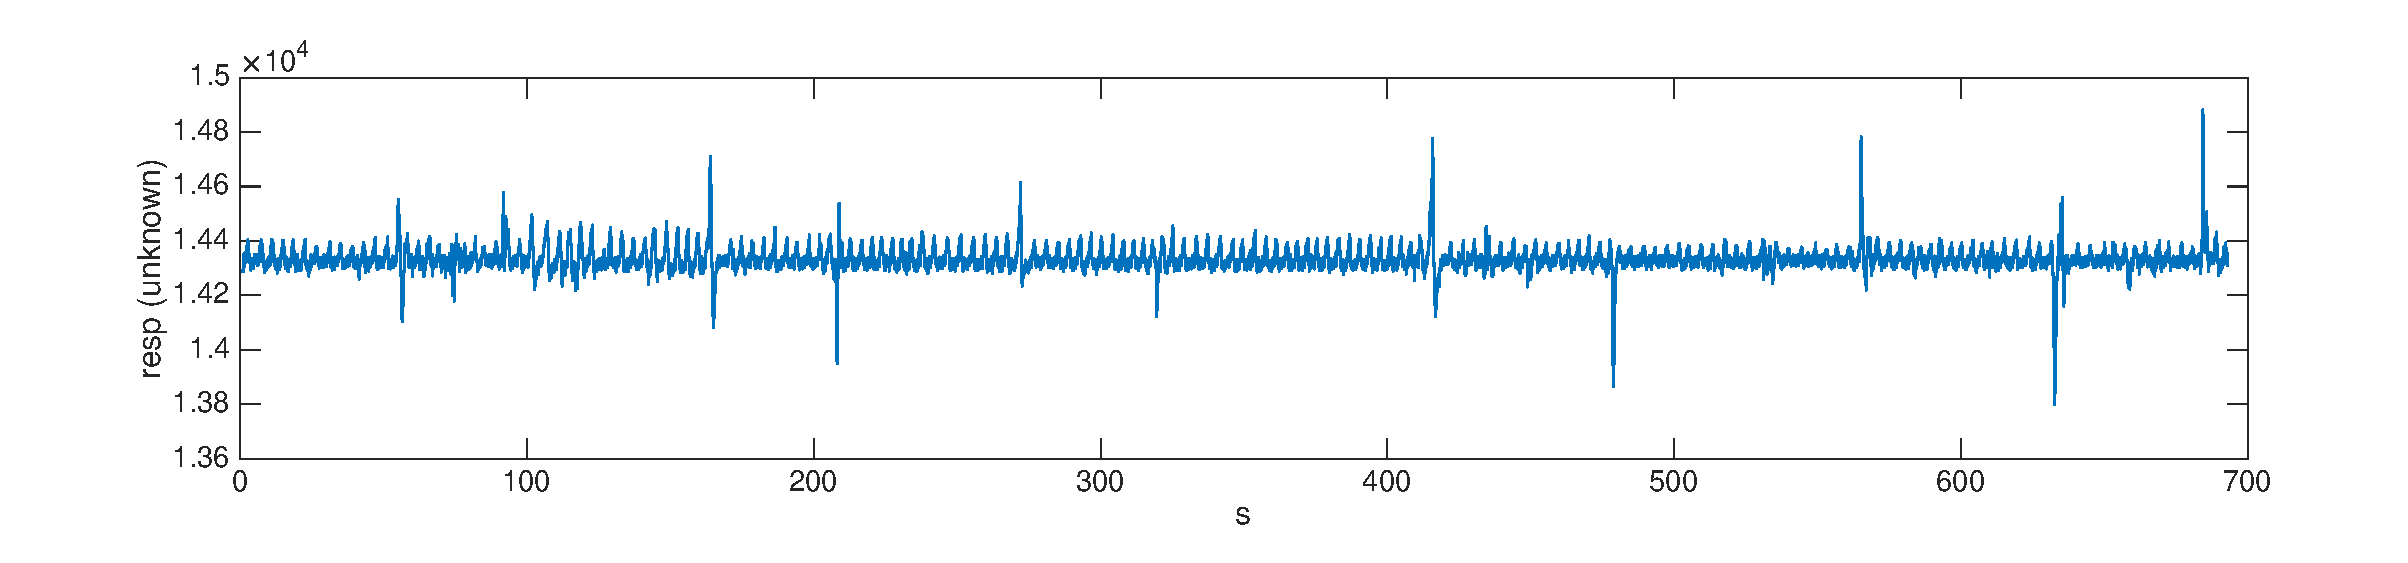
\includegraphics[width=0.9\textwidth]{data/raw-resp}
  \DeclareGraphicsExtensions.
  \caption{The respiration signal.} \label{fig:raw-resp}
\end{figure}

\section{Test on the script}

We have received the script of \textit{Amin and Faghih}'s work \cite{amin2019robust}. The original dataset is stored in \texttt{s.mat}. The pre-processing and phasic extraction are done by \texttt{pre\_processing\_auditory\_stimulation}, then the extracted phasic signal is deconvolved by \texttt{Exp\_on\_real\_data\_3\_channel\_4\_25\_2019}.

\begin{figure}[htbp]
  \centering
  \subfigure[GSR collected on thenar/hypothenar.]{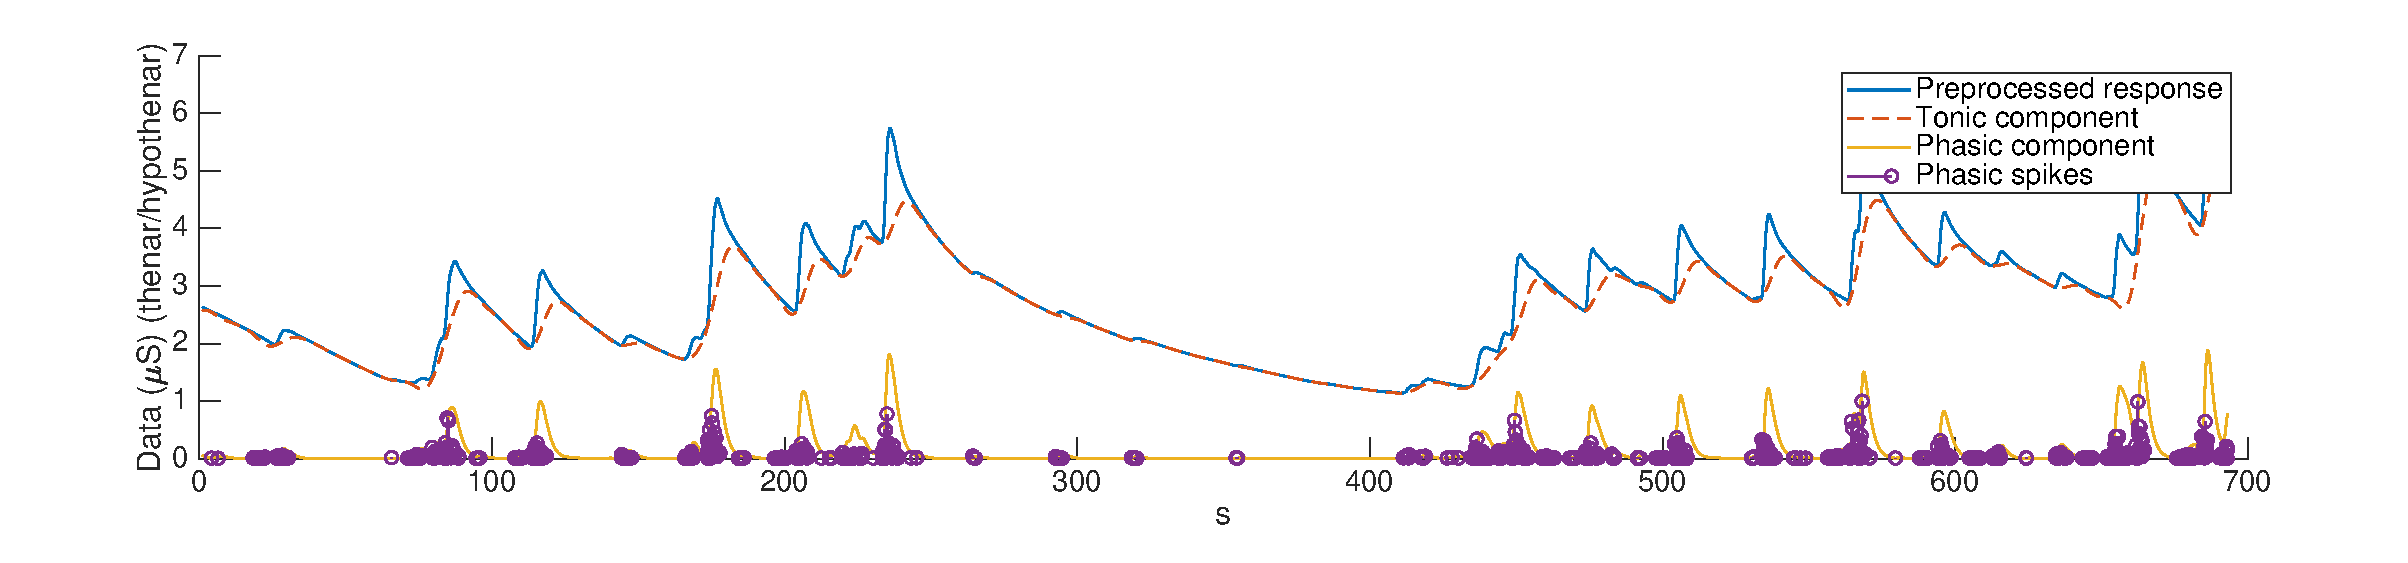
\includegraphics[width=0.9\textwidth]{data/sep-thenar}}
  \subfigure[GSR collected on volar middle phalanx.]{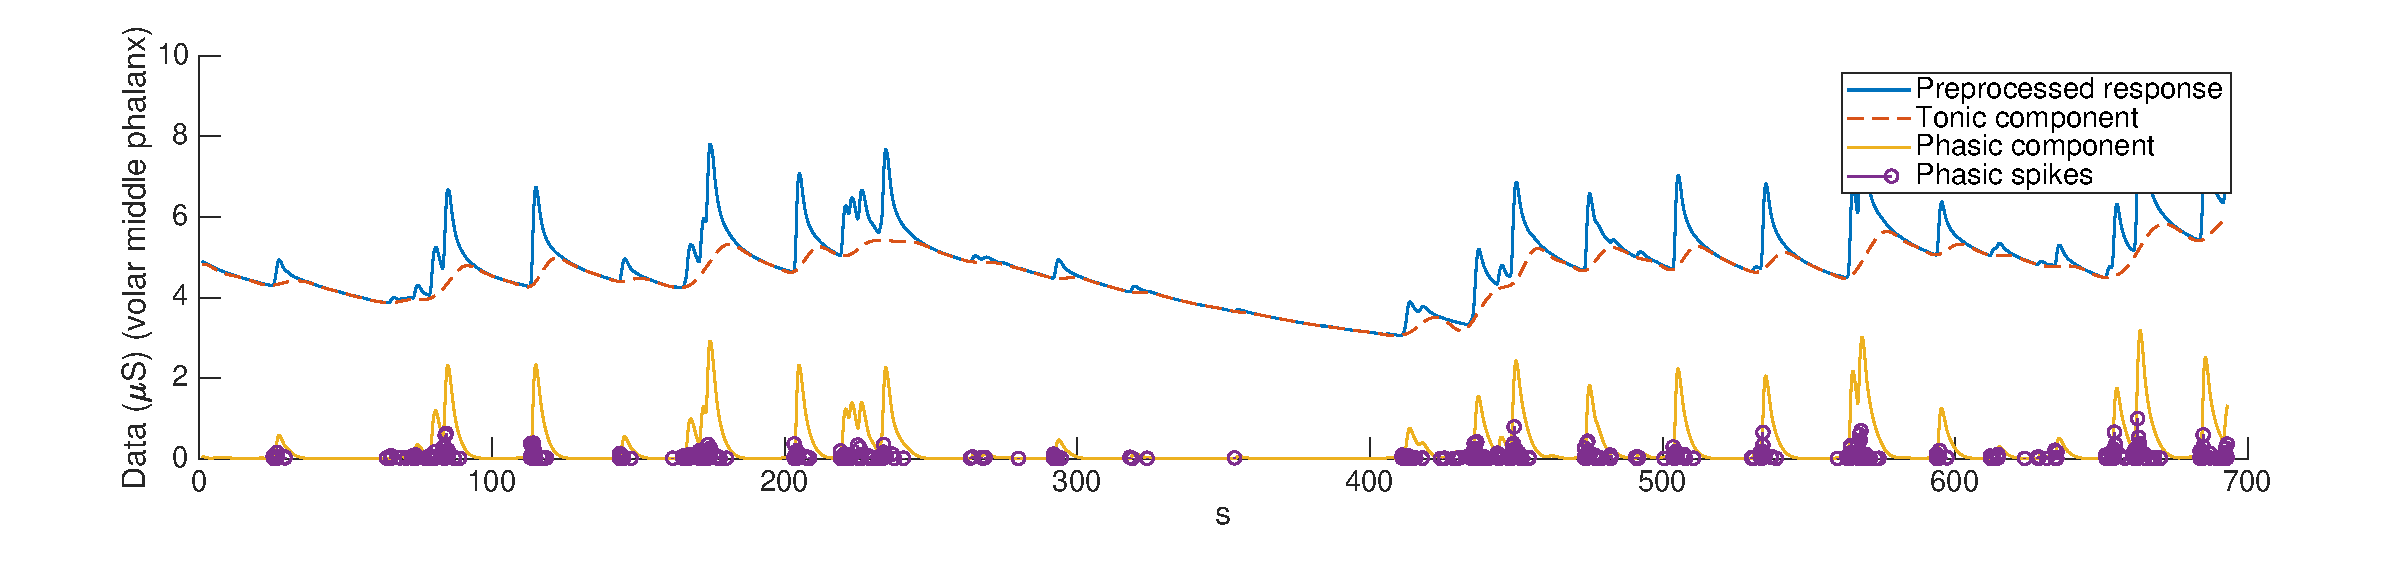
\includegraphics[width=0.9\textwidth]{data/sep-volar}}
  \subfigure[GSR collected on medial plantar surface.]{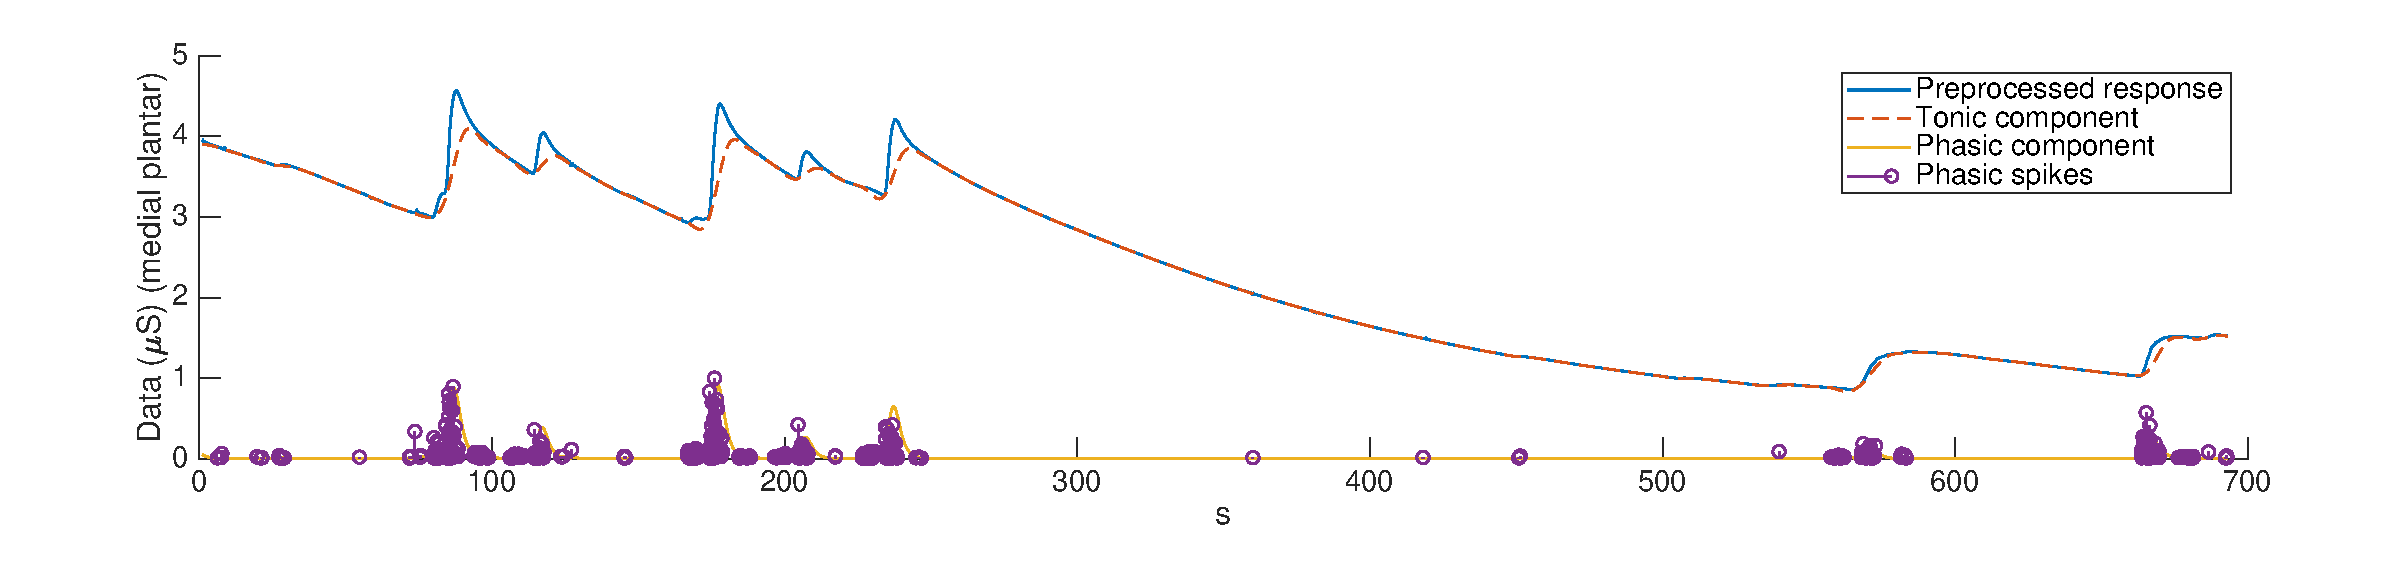
\includegraphics[width=0.9\textwidth]{data/sep-medial} \label{fig:sep-signal-medial}}
  \DeclareGraphicsExtensions.
  \DeclareGraphicsExtensions.
  \caption{The separated signals of the $6^{\mathrm{th}}$ data.} \label{fig:sep-signal}
\end{figure}

The pre-processing is aimed at removing the outliers in the raw signal. This is a pure technical method. The algorithm could be divided into 3 steps:

\begin{enumerate}
  \item Find the super abnormal peaks and the lower abnormal peaks with a threshold.
  \item The 100 points around the abnormal peaks are replaced by the spline integration result.
  \item The data is finally filtered by a low-pass filter.
\end{enumerate}

Then the data is processed by cvxEDA~\cite{greco2015cvxeda}. The cvxEDA is designed for deconvolution with component separation. It is used for separating the tonic component from the raw signal. The separation is performed on each channel for each data. To show the results, we design a function \texttt{show\_arranged\_dataset}. The separated signals are plotted in \autoref{fig:sep-signal}. Note that in \autoref{fig:sep-signal-medial}, since the data is pre-processed, the outliers are removed compared to \autoref{fig:raw-medial}.

Finally, after running the script \texttt{Exp\_on\_real\_data\_3\_channel\_4\_25\_2019}, we could use another script \texttt{plot\_figure\_for\_journal} to display the final deconvolved results. \autoref{fig:deconv} show the results within 200 seconds. The multichannel deconvolution is solely performed on phasic components. The scatters represent the input phasic components, and the green lines represent the reconstructed signals with the extracted spikes.

\begin{figure}[htbp]
  \centering
  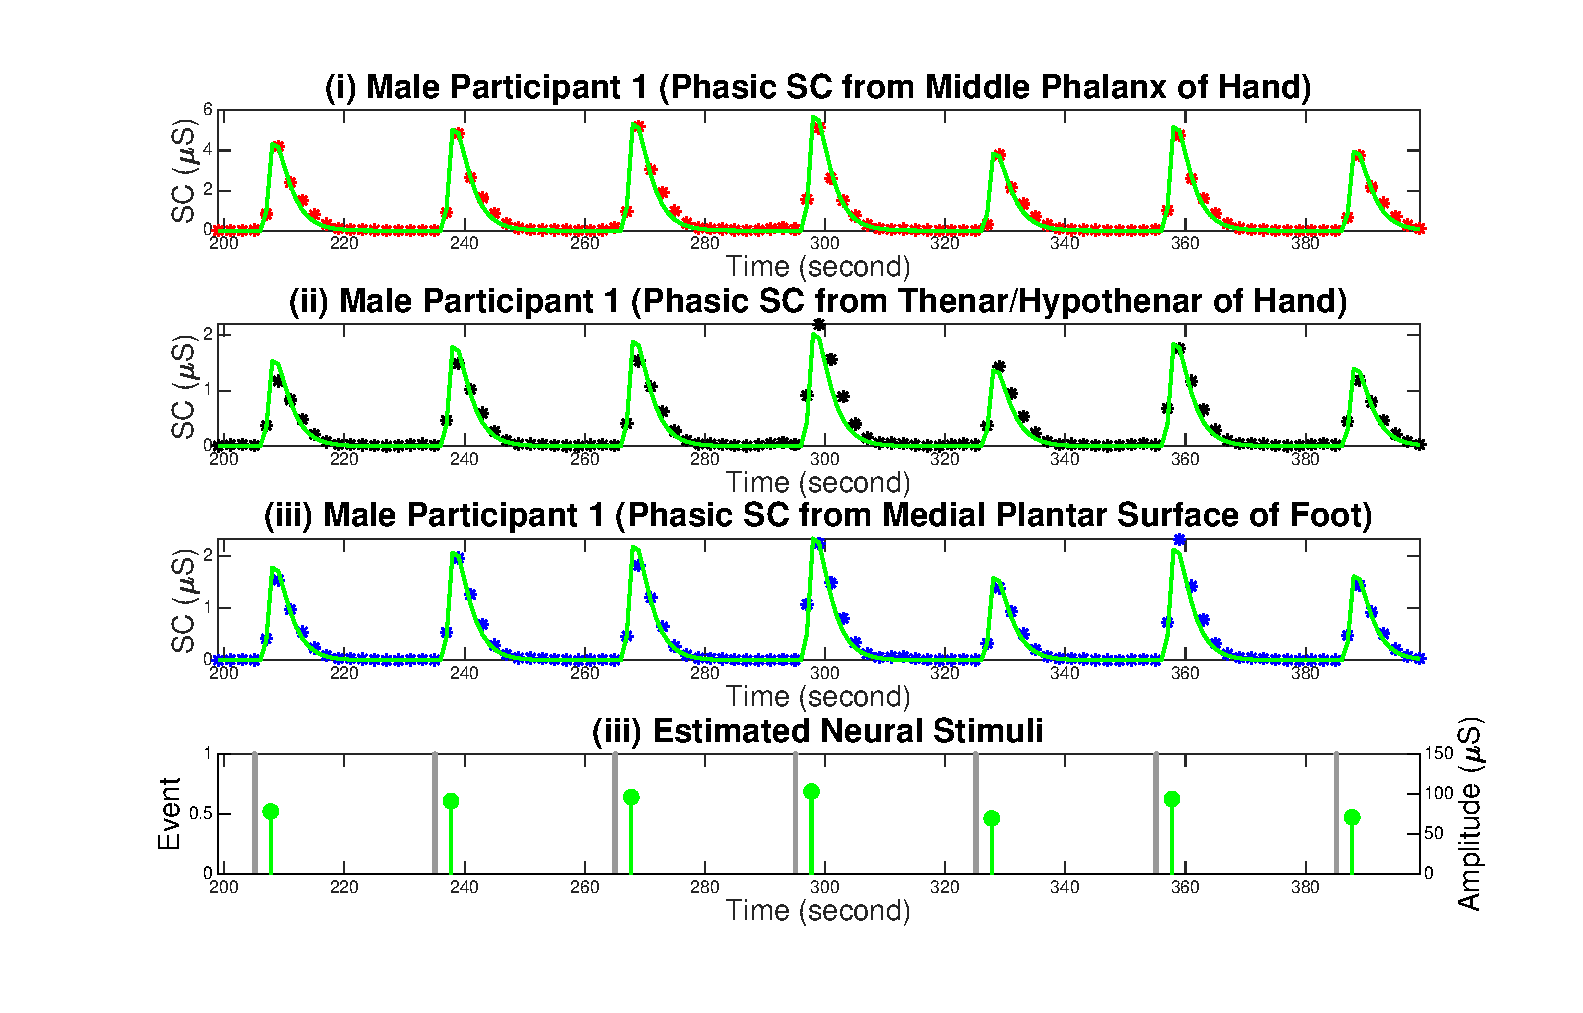
\includegraphics[width=0.9\textwidth]{data/deconv}
  \DeclareGraphicsExtensions.
  \caption{Results of the deconvolution.} \label{fig:deconv}
\end{figure}

\bibliographystyle{ieeetr}
\bibliography{ref}

\end{document}
